\documentclass[11pt]{article}

\usepackage[margin=1in]{geometry}
\usepackage{amsmath,amssymb,amsthm}
\usepackage{booktabs}
\usepackage{enumitem}
\usepackage{hyperref}
\usepackage{xcolor}
\usepackage{tikz}
\usetikzlibrary{arrows.meta,positioning,fit,calc}

\title{Lecture~6 Study Notes:\\Sequences, Recurrent Neural Networks,\\and Sequence-to-Sequence Learning}
\author{Deep Learning Notes\\
\small Ground-up intuitions and worked examples\\[0.35em]
\small Formation borrows heavily from the
\href{https://r-three.github.io/deep-learning-lecture-notes/}{original course website (CSC2516)}}
\date{}

\newtheorem*{clarification}{Clarification}

\begin{document}
\maketitle

\begin{abstract}
These notes develop \textbf{sequences, recurrent networks, and
sequence-to-sequence models} from first principles, with the questions,
intuitions, and metaphors that came up while studying the lecture. A
sequence factors by the chain rule into next-element predictions. Storing a
separate distribution for every prefix is a giant lookup table; a recurrent
net replaces that table by one shared set of weights and a hidden state
that stands in for the prefix. Words enter the net as columns of a learned
\textbf{embedding matrix}. Backpropagation through time shows why those
shared weights explode or vanish. The \textbf{LSTM} answers with a private
notebook and three dimmer switches. The same decoder LSTM is then counted
carefully in a sequence-to-sequence model, and four practice problems are
worked in full. Content formation borrows heavily from the original
\href{https://r-three.github.io/deep-learning-lecture-notes/lectures/06-sequences-recurrent-neural-networks-and-sequence-to-sequence-learning.html}{Lecture~6 notes (CSC2516)}.
\end{abstract}

\tableofcontents
\vspace{1em}

%----------------------------------------------------------------------
\section{Sequences and the Chain Rule}
%----------------------------------------------------------------------

Almost every model so far predicts one output from one input. A
\emph{sequence} is different: it is an ordered series of random variables
\(\mathbf{x}_1,\mathbf{x}_2,\ldots,\mathbf{x}_T\). The order is part of the
data. A spectrogram is a sequence of spectra, a video is a sequence of
frames, and a sentence is a sequence of words. Shuffle the measurements in
time and the series is no longer the same object.

The chain rule writes the joint as a product of next-element conditionals:
\begin{equation}
\label{eq:chain}
\begin{aligned}
p(\mathbf{x}_1,\ldots,\mathbf{x}_T)
&=
p(\mathbf{x}_1)\,
p(\mathbf{x}_2\mid\mathbf{x}_1)\,
p(\mathbf{x}_3\mid\mathbf{x}_2,\mathbf{x}_1)
\cdots
p(\mathbf{x}_T\mid\mathbf{x}_{T-1},\ldots,\mathbf{x}_1).
\end{aligned}
\end{equation}
Any collection of random variables factors this way. The sequence matters
because \emph{this} order is the natural one: when the first thing we see
is \(\mathbf{x}_1\), asking for \(p(\mathbf{x}_1)\) is meaningful, and then
asking for \(p(\mathbf{x}_2\mid\mathbf{x}_1)\) is meaningful. Asking for
\(p(\mathbf{x}_3\mid\mathbf{x}_{10})\) conditions on something we have not
observed yet.

For the sentence ``the cat sat'',
\[
p(\text{the cat sat})
=
p(\text{the})\,
p(\text{cat}\mid\text{the})\,
p(\text{sat}\mid\text{the, cat}).
\]

\subsection{One model, every factor}

Each factor in~\eqref{eq:chain} is a conditional distribution of one element
given a prefix. Training a separate model for \(p(\mathbf{x}_1)\), another
for \(p(\mathbf{x}_2\mid\mathbf{x}_1)\), and so on, does not scale. The
practical object is a \emph{single} model of
\[
p(\mathbf{x}_t\mid\mathbf{x}_{t-1},\ldots,\mathbf{x}_1)
\]
that accepts a prefix of any length. That one model supplies every factor.
Recurrent networks are the first architecture in the course that does this.
Transformers will do it later, without the recurrence.

\subsection{Autoregressive sampling}

A classifier predicts \(\mathbf{y}\) given \(\mathbf{x}\). A model of the
joint over sequences can also \emph{generate}. Sample left to right, feeding
each draw back in as the next prefix:
\begin{enumerate}[leftmargin=*]
  \item draw \(\mathbf{x}_1\sim p(\mathbf{x}_1)\);
  \item draw \(\mathbf{x}_2\sim p(\mathbf{x}_2\mid\mathbf{x}_1)\), using the
        \(\mathbf{x}_1\) just sampled;
  \item draw \(\mathbf{x}_3\sim p(\mathbf{x}_3\mid\mathbf{x}_2,\mathbf{x}_1)\),
        and continue until the sequence is finished.
\end{enumerate}
This is \textbf{autoregressive sampling}. Scoring an existing sequence is
the same factorization with the observed tokens plugged in: multiply the
conditionals. Generating and scoring are two uses of one next-element model.

\begin{quote}
\emph{One-line intuition (kept throughout).}
The prefix is the input. The next element is a classification problem.
The hidden state is a running summary of that prefix, so the parameter
count does not grow with \(T\).
\end{quote}

%----------------------------------------------------------------------
\section{Worked Count: A Separate Distribution per Prefix}
%----------------------------------------------------------------------

\begin{clarification}
The vocabulary has 3 words and every sequence has exactly 4 words. An
autoregressive model stores, for every possible prefix (including the empty
prefix), a separate categorical distribution over the next word. A
categorical distribution over 3 words has 2 free parameters. How many free
parameters does the model have in total?
\end{clarification}

This is the lookup-table version of~\eqref{eq:chain}, before any weight
sharing. Call the words \(a,b,c\). A prefix is the beginning of a sequence,
and the model needs a distribution only when a next word still has to be
predicted. Sequences stop at length 4, so the prefixes have length
\(0,1,2,\) or \(3\).

\subsection{Why one distribution contributes 2 numbers}

One next-word distribution is three probabilities that add to 1:
\[
p_a+p_b+p_c=1, \qquad p_a,p_b,p_c\ge 0.
\]
Choose \(p_a\) and \(p_b\). The third is forced:
\[
p_c=1-p_a-p_b.
\]
If \(p_a=0.5\) and \(p_b=0.2\), then \(p_c=0.3\) is not a third choice. A
categorical distribution over 3 words has \textbf{2 free parameters}. The
same pair of numbers is stored again, separately, at every other prefix.
The prefix \(ab\) has its own pair, for example
\(p(a\mid ab)=0.1\) and \(p(b\mid ab)=0.7\), which forces
\(p(c\mid ab)=0.2\). Those two numbers are a different pair from the empty
prefix's pair.

\subsection{How many prefixes}

\begin{center}
\begin{tabular}{@{}lll@{}}
\toprule
Prefix length & What it predicts & How many prefixes \\
\midrule
0 (empty) & \(x_1\) & \(3^0=1\) \\
1 & \(x_2\) & \(3^1=3\), namely \(a,b,c\) \\
2 & \(x_3\) & \(3^2=9\), namely \(aa,ab,\ldots,cc\) \\
3 & \(x_4\) & \(3^3=27\) \\
\bottomrule
\end{tabular}
\end{center}

\[
1+3+9+27=40
=
\sum_{k=0}^{3} 3^k
=
\frac{3^4-1}{3-1}.
\]
Each of the 40 tables stores 2 free numbers:
\[
40\times 2=80.
\]
The factor of 2 is ``two choices per table,'' not a second copy of the
table. The factor of 40 is ``one table per prefix.''

In general, vocabulary size \(|V|\) and length \(T\) give
\[
\frac{|V|^T-1}{|V|-1}
\]
prefixes, each with \(|V|-1\) free probabilities. Here \(|V|=3\) and \(T=4\)
already costs 80 numbers. Most long prefixes never appear in training text,
so their rows have no data. The recurrent net in the next sections replaces
this table by one shared set of weights. The hidden state \(h_t\) stands in
for the prefix, and the parameter count stays fixed when \(T\) grows.

%----------------------------------------------------------------------
\section{From a Word to a Vector}
%----------------------------------------------------------------------

A word is a string. There is no sensible way to multiply the string
\(\texttt{cat}\) by a weight matrix. Mapping text into the network has
three steps: an index, a one-hot vector, and a short learned vector called
an \textbf{embedding}.

\subsection{Index, then one-hot}

A \textbf{tokenizer} fixes a vocabulary \(V\) and gives each word an integer
index. The index is only a name. In a four-word baby vocabulary,

\begin{center}
\begin{tabular}{@{}lc@{}}
\toprule
word & index \\
\midrule
the & 1 \\
cat & 2 \\
sat & 3 \\
dog & 4 \\
\bottomrule
\end{tabular}
\end{center}

Feeding the raw index into a matrix would be a mistake. If ``the'' is 1 and
``cat'' is 2, multiplying by 2 treats ``cat'' as twice ``the.'' Words have
no such size. The remedy is the same one used for class labels: a
\textbf{one-hot vector}, with a single 1 in the index position and zeros
elsewhere. Its length is \(|V|\):
\begin{align*}
\text{the} &= [1,\ 0,\ 0,\ 0], &
\text{cat} &= [0,\ 1,\ 0,\ 0], \\
\text{sat} &= [0,\ 0,\ 1,\ 0], &
\text{dog} &= [0,\ 0,\ 0,\ 1].
\end{align*}
Every one-hot vector has the same length and the same norm. No word is
numerically larger than another.

\subsection{The embedding matrix selects a column}

Suppose each word is represented by 3 numbers (a real model uses hundreds).
The \textbf{embedding matrix} \(W\) has 3 rows, one per embedding
coordinate, and 4 columns, one per vocabulary word. Invent a matrix the
model might have learned:
\[
\begin{array}{c@{\;}c}
 &
 \begin{array}{cccc}
 \scriptstyle\text{the} & \scriptstyle\text{cat} &
 \scriptstyle\text{sat} & \scriptstyle\text{dog}
 \end{array}
 \\[0.3em]
W =
 &
\begin{bmatrix}
0.2 & 0.9 & 0.1 & 0.8 \\
0.1 & 0.7 & 0.3 & 0.6 \\
-0.4 & -0.2 & 0.5 & -0.1
\end{bmatrix}
\end{array}
\]
The one-hot vector for ``cat'' is \([0,1,0,0]^\top\). Matrix--vector
multiplication copies out the column where the 1 sits and wipes out the
others:
\[
W
\begin{bmatrix}0\\1\\0\\0\end{bmatrix}
=
0\cdot(\text{col 1})
+1\cdot(\text{col 2})
+0\cdot(\text{col 3})
+0\cdot(\text{col 4})
=
\begin{bmatrix}0.9\\0.7\\-0.2\end{bmatrix}.
\]
That column is the \textbf{word embedding} of ``cat.'' In code this is an
index, \(W_{:,2}\). The product and the index do the same thing. The four
embeddings in this baby matrix are
\begin{align*}
\text{the}&=[0.2,\ 0.1,\ -0.4], &
\text{cat}&=[0.9,\ 0.7,\ -0.2], \\
\text{sat}&=[0.1,\ 0.3,\ 0.5], &
\text{dog}&=[0.8,\ 0.6,\ -0.1].
\end{align*}
``cat'' and ``dog'' are close. ``the'' is far from both. The sentence
``the cat sat'' becomes three short vectors, one per step, and those
vectors are what the network sees:
\begin{align*}
t=1,\ \text{the} &\mapsto [0.2,\ 0.1,\ -0.4], \\
t=2,\ \text{cat} &\mapsto [0.9,\ 0.7,\ -0.2], \\
t=3,\ \text{sat} &\mapsto [0.1,\ 0.3,\ 0.5].
\end{align*}

In the RNN of Section~\ref{sec:vanilla}, the current input \(x_t\) is this
one-hot vector, and the first weight matrix \(W_x\) \emph{is} the embedding
matrix. The product \(W_x x_t\) is the current word's embedding.

Next-word prediction is then \(|V|\)-way classification. With 4 words the
network ends in a softmax with 4 scores. The sizes in the baby model are:
one-hot input of length 4, embedding matrix \(3\times 4\), embedding of
length 3, softmax output of length 4.

\paragraph{Why a learned vector beats the index.}
Words that play similar roles get pushed toward similar columns, because
that helps predict the next word. A famous illustration, with made-up
2-dimensional numbers:
\begin{align*}
\text{king}&=[0.9,\ 0.8], &
\text{man}&=[0.7,\ 0.2], \\
\text{woman}&=[0.7,\ -0.2], &
\text{queen}&=[0.9,\ 0.4].
\end{align*}
\[
\text{king}-\text{man}+\text{woman}
=
[0.9,0.8]-[0.7,0.2]+[0.7,-0.2]
=
[0.9,0.4],
\]
which lands on ``queen.'' Nobody stored that equation. It falls out of the
learned columns (Mikolov et al., 2013).

\begin{clarification}
How do the numbers in the embedding matrix get decided?
\end{clarification}

They are not chosen by hand. At the start of training every entry of \(W\)
is a small random number. The training signal is next-word prediction. For
``the cat sat'' the model is shown a prefix and asked for the following
word:

\begin{center}
\begin{tabular}{@{}ll@{}}
\toprule
Prefix it sees & Word it must predict \\
\midrule
the & cat \\
the cat & sat \\
\bottomrule
\end{tabular}
\end{center}

The output is a softmax over the vocabulary. Cross-entropy is small when
the score on the true next word is high. Backpropagation sends a gradient
from that loss back into the only column that this example selected. If the
current word is ``the,'' only the ``the'' column of \(W\) has a nonzero
gradient on this step, because the other one-hot entries were 0. A gradient
step
\[
W\leftarrow W-\eta\,\frac{\partial\mathcal{L}}{\partial W}
\]
nudges that column. After many sentences, words that show up in similar
contexts get nudged in similar ways, so their columns end up close.

\begin{clarification}
So the word embedding is learned via the RNN?
\end{clarification}

In this lecture, yes. The embedding matrix is one of the RNN's own weight
matrices, \(W_x\), and it is trained in the same loop as the rest of the
network. There is no separate embedding stage. A column is a useful
embedding after training because using it that way made the next-word loss
smaller.

\begin{clarification}
How does that compare to word2vec?
\end{clarification}

Same kind of object: a column in a matrix that turns a word into a short
vector. The training setup is different.

Word2vec looks at a small window. In ``the cat sat,'' with one word on each
side of the center, skip-gram asks: given ``cat,'' predict the neighbors
``the'' and ``sat.'' The model is shallow,
\[
\text{``cat''}
\;\rightarrow\;
\text{one column of the embedding matrix}
\;\rightarrow\;
\text{softmax over the vocabulary}.
\]
There is no hidden state and no recurrence. After training, the rest of the
model is discarded. The columns are the result. The king\(-\)man\(+\)woman
pattern in the lecture comes from this training setup.

The RNN's question is the next word given the whole prefix, and the
embedding is only the input to that computation:
\[
\operatorname{embed}(\text{the})\rightarrow h_1,
\qquad
\operatorname{embed}(\text{cat})\rightarrow h_2,
\]
where \(h_2\) also depends on \(h_1\), and the softmax on \(h_2\) is trained
to put its mass on ``sat.'' The column stays attached to the language
model. Context lives in the hidden state, not only in which columns happen
to be near each other.

\begin{center}
\begin{tabular}{@{}lll@{}}
\toprule
 & Word2vec & RNN embedding in this lecture \\
\midrule
What is trained & the embedding matrix & \(W_x\) plus recurrent and output weights \\
Prediction & a nearby word in a fixed window & the next word given the whole prefix \\
Where context lives & nearby columns of the matrix & the hidden state \(h_t\) \\
What you keep & the columns, used later as features & the full network \\
\bottomrule
\end{tabular}
\end{center}

%----------------------------------------------------------------------
\section{The Vanilla Recurrent Network}
\label{sec:vanilla}
%----------------------------------------------------------------------

Start from a one-hidden-layer network and make the smallest change that
accepts a prefix of any length. The feedforward net, with \(W_x\) reserved
for the input weights, is
\[
\mathbf{h}=\sigma(W_x\mathbf{x}+\mathbf{b}_h),
\qquad
\mathbf{o}=W_o\mathbf{h}+\mathbf{b}_o.
\]
Make the hidden state a sequence, and add a recurrent connection so step
\(t\) depends on step \(t-1\):
\begin{equation}
\label{eq:vanilla}
\mathbf{h}_t
=
\sigma(W_x\mathbf{x}_t+W_h\mathbf{h}_{t-1}+\mathbf{b}_h),
\qquad
\mathbf{o}_t
=
W_o\mathbf{h}_t+\mathbf{b}_o.
\end{equation}
The new term is \(W_h\mathbf{h}_{t-1}\). Start from an initial state
\(\mathbf{h}_0\) (usually zeros, or a learned vector) and feed
\(\mathbf{x}_1\) to get \(\mathbf{h}_1\), then \(\mathbf{x}_2\) together
with the retained \(\mathbf{h}_1\) to get \(\mathbf{h}_2\), and so on.

Because \(\mathbf{h}_t\) is computed from \(\mathbf{x}_t\) and
\(\mathbf{h}_{t-1}\), and \(\mathbf{h}_{t-1}\) from \(\mathbf{x}_{t-1}\) and
\(\mathbf{h}_{t-2}\), the state \(\mathbf{h}_t\) depends on every past
input. It is a summary of the prefix up to step \(t\): not a literal
sentence, but a vector that carries information about all the inputs so far.

Two properties follow.
\begin{itemize}[leftmargin=*]
  \item \textbf{Any length.} A longer sequence means more updates of
        \(\mathbf{h}_t\). The input dimension of \(W_x\) stays fixed.
  \item \textbf{A fixed parameter list.} The same \(W_x\), \(W_h\),
        \(\mathbf{b}_h\), \(W_o\), and \(\mathbf{b}_o\) are reused at every
        position, just as a convolution reuses one filter. Growing \(T\)
        does not add parameters. The vocabulary size is fixed once chosen:
        \(\mathbf{x}_t\) has dimension \(|V|\), so \(W_x\) has a matching
        number of columns.
\end{itemize}

As written, \eqref{eq:vanilla} emits an output \(\mathbf{o}_t\) at every
step, which is what next-element prediction wants. For sequence
classification, feed the whole sequence and read a single output from the
final state \(\mathbf{h}_T\).

The network introduces no new kind of operation: nonlinearities, bias
additions, and matrix multiplies. Automatic differentiation trains it.
What changes is the shape of the graph once it is unrolled in time.

%----------------------------------------------------------------------
\section{Backpropagation through Time}
\label{sec:bptt}
%----------------------------------------------------------------------

Picture the recurrence unrolled: the same layer applied at
\(t=1,2,\ldots,T\), then ordinary backpropagation on that long graph.
Backpropagation on the unrolled graph is \textbf{backpropagation through
time}. Write the hidden update as \(f\) and the output map as \(g\),
\[
\mathbf{h}_t=f(\mathbf{x}_t,\mathbf{h}_{t-1},W_h),
\qquad
\mathbf{o}_t=g(\mathbf{h}_t,W_o),
\]
and put a loss at every step,
\[
\mathcal{L}
=
\frac{1}{T}\sum_{t=1}^{T}\ell(\mathbf{y}_t,\mathbf{o}_t).
\]
The parameter that makes this different from a feedforward net is \(W_h\),
because the same matrix is used at every step. By linearity and the chain
rule,
\[
\frac{\mathrm{d}\mathcal{L}}{\mathrm{d}W_h}
=
\frac{1}{T}\sum_{t=1}^{T}
\frac{\mathrm{d}\ell}{\mathrm{d}\mathbf{o}_t}
\frac{\mathrm{d}\mathbf{o}_t}{\mathrm{d}\mathbf{h}_t}
\frac{\mathrm{d}\mathbf{h}_t}{\mathrm{d}W_h}.
\]
The first factor is a softmax cross-entropy gradient. The second is
\(W_o\). The third factor is the hard one.

\subsection{The direct path and the indirect path}

\(W_h\) affects \(\mathbf{h}_t\) twice: directly, because \(\mathbf{h}_t\) is
computed with \(W_h\), and indirectly, because \(\mathbf{h}_t\) depends on
\(\mathbf{h}_{t-1}\), which itself depends on \(W_h\). When a variable
reaches another through two paths, add the derivatives:
\begin{equation}
\label{eq:bptt-recursion}
\frac{\mathrm{d}\mathbf{h}_t}{\mathrm{d}W_h}
=
\frac{\partial f}{\partial W_h}
+
\frac{\partial f}{\partial\mathbf{h}_{t-1}}
\frac{\mathrm{d}\mathbf{h}_{t-1}}{\mathrm{d}W_h}.
\end{equation}
The last factor has the same shape one step earlier. Unrolling the
recursion produces an immediate term plus a sum of products of the
step-to-step Jacobians \(\partial f/\partial\mathbf{h}_{j-1}\).

For a \emph{linear} vanilla RNN,
\(f=W_x\mathbf{x}_t+W_h\mathbf{h}_{t-1}+\mathbf{b}_h\), each
step-to-step factor is the same matrix \(W_h\), and
\begin{equation}
\label{eq:linear-bptt}
\frac{\mathrm{d}\mathbf{h}_t}{\mathrm{d}W_h}
=
\mathbf{h}_{t-1}
+
\sum_{i=1}^{t-1}
\Bigl(\prod_{j=i+1}^{t} W_h\Bigr)
\mathbf{h}_{i-1}.
\end{equation}
The product \(\prod W_h\) is the same matrix multiplied by itself over and
over. A chain of identical matrix multiplies grows without bound or shrinks
toward zero according to the eigenvalues of \(W_h\). Viewing the unrolled
RNN as a deep net whose layers share one weight matrix makes the point:
exploding and vanishing gradients are especially severe here, because the
matrices in the product are not merely similar. They are the same matrix.

\subsection{Worked gradient: scalar linear RNN}
\label{sec:q3}

\begin{clarification}
A scalar linear RNN has \(h_t=w h_{t-1}+x_t\) with \(w=-2\) and \(h_0=0\).
The loss is \(\mathcal{L}=\sum_{t=1}^{6} h_t\). What is
\(\partial\mathcal{L}/\partial x_1\)?
\end{clarification}

This is~\eqref{eq:linear-bptt} in the simplest setting: the shared weight is
a number, and the question asks how the first input flows into every later
state. Unroll from \(h_0=0\):
\begin{align*}
h_1 &= x_1, \\
h_2 &= w x_1+x_2, \\
h_3 &= w^2 x_1+w x_2+x_3, \\
h_4 &= w^3 x_1+\cdots, \\
h_5 &= w^4 x_1+\cdots, \\
h_6 &= w^5 x_1+\cdots.
\end{align*}
Each new step multiplies the old state by \(w\), so the copy of \(x_1\)
inside \(h_t\) is \(w^{t-1}x_1\).

The loss adds the six states, so the derivative adds six derivatives:
\[
\frac{\partial\mathcal{L}}{\partial x_1}
=
\frac{\partial h_1}{\partial x_1}
+\cdots+
\frac{\partial h_6}{\partial x_1}.
\]
Differentiate one state at a time. \(h_1=x_1\), so
\(\partial h_1/\partial x_1=1\). Next,
\(h_2=wx_1+x_2\). The input \(x_2\) does not depend on \(x_1\), so
\(\partial h_2/\partial x_1=w\). One more step multiplies by \(w\) again:
\(\partial h_3/\partial x_1=w^2\). Continuing,
\[
\frac{\partial\mathcal{L}}{\partial x_1}
=
1+w+w^2+w^3+w^4+w^5.
\]
The \(1\) is \(w^0\), from \(h_1\). The last power is \(w^5\), from \(h_6\),
because \(x_1\) passes through five multiplications by \(w\) to reach step
6. Substitute \(w=-2\):
\begin{align*}
1&=1, &
w&=-2, &
w^2&=4, &
w^3&=-8, &
w^4&=16, &
w^5&=-32.
\end{align*}
\[
1-2+4-8+16-32=-21.
\]
The same sum is the geometric series \((1-w^6)/(1-w)\):
\[
\frac{1-(-2)^6}{1-(-2)}
=
\frac{1-64}{3}
=
-21.
\]
The terms grow by 2 at every step because \(|w|>1\). That is the exploding
gradient in scalar form: an input at step 1 still has a large effect on the
loss at step 6. The alternating sign is the negative weight.

\subsection{Worked gradient: scalar ReLU RNN}
\label{sec:q4}

\begin{clarification}
A scalar ReLU RNN has \(h_t=\mathrm{ReLU}(w h_{t-1}+x_t)\) with \(h_0=0\)
and \(w=2\). The inputs are \((x_1,\ldots,x_6)=(1,1,-8,2,1,1)\) and the loss
is \(\mathcal{L}=\sum_{t=1}^{6}h_t\). What is \(\mathrm{d}\mathcal{L}/\mathrm{d}w\)?
ReLU has slope \(1\) for a positive input and slope \(0\) for a negative
input, and no pre-activation here is exactly \(0\).
\end{clarification}

Write the pre-activation \(z_t=w\cdot h_{t-1}+x_t\), so
\(h_t=\mathrm{ReLU}(z_t)\). Run the recurrence forward before any
derivative.

\begin{center}
\begin{tabular}{@{}ccccc@{}}
\toprule
\(t\) & \(x_t\) & \(z_t=w h_{t-1}+x_t\) & sign & \(h_t\) \\
\midrule
1 & \(1\)  & \(2\cdot 0+1=1\)   & \(>0\) & \(1\) \\
2 & \(1\)  & \(2\cdot 1+1=3\)   & \(>0\) & \(3\) \\
3 & \(-8\) & \(2\cdot 3-8=-2\) & \(<0\) & \(0\) \\
4 & \(2\)  & \(2\cdot 0+2=2\)   & \(>0\) & \(2\) \\
5 & \(1\)  & \(2\cdot 2+1=5\)   & \(>0\) & \(5\) \\
6 & \(1\)  & \(2\cdot 5+1=11\)  & \(>0\) & \(11\) \\
\bottomrule
\end{tabular}
\end{center}

The six slopes are \(1,1,0,1,1,1\). The loss is the sum of the hidden
states, so
\[
\frac{\mathrm{d}\mathcal{L}}{\mathrm{d}w}
=
\frac{\mathrm{d}h_1}{\mathrm{d}w}+\cdots+\frac{\mathrm{d}h_6}{\mathrm{d}w}.
\]
The weight \(w\) is reused at every step, and each \(h_t\) is built from
\(h_{t-1}\). Both effects count. This is the scalar version
of~\eqref{eq:bptt-recursion}, with an extra ReLU slope.

On a positive step, \(h_t=z_t\), so the derivatives match. On a negative
step, \(h_t\) is the constant \(0\), so its derivative is \(0\).
Differentiating the product \(w\cdot h_{t-1}\) has two pieces, because both
factors can change with \(w\):
\begin{itemize}[leftmargin=*]
  \item \(w\) changes while \(h_{t-1}\) is held at its current value. That
        piece contributes \(h_{t-1}\).
  \item \(h_{t-1}\) changes because earlier steps used \(w\), and that
        change is then multiplied by the current \(w\). That piece
        contributes \(w\cdot\mathrm{d}h_{t-1}/\mathrm{d}w\).
\end{itemize}
The input \(x_t\) is a fixed number. Combining the two pieces with the ReLU
slope,
\begin{equation}
\label{eq:relu-bptt}
\frac{\mathrm{d}h_t}{\mathrm{d}w}
=
\mathrm{ReLU}'(z_t)
\cdot
\Bigl(
h_{t-1}
+
w\cdot\frac{\mathrm{d}h_{t-1}}{\mathrm{d}w}
\Bigr).
\end{equation}
The given \(h_0=0\) was not computed from \(w\), so
\(\mathrm{d}h_0/\mathrm{d}w=0\). Apply~\eqref{eq:relu-bptt} one step at a
time.

\(t=1\). Slope \(1\), previous state \(0\), previous derivative \(0\):
\[
\frac{\mathrm{d}h_1}{\mathrm{d}w}
=
1\cdot(0+2\cdot 0)=0.
\]
\(h_1=1\) came from \(2\cdot 0+1\). Changing \(w\) does not change
\(2\cdot 0\).

\(t=2\). Slope \(1\), and \(h_1=1\) does not move with \(w\):
\[
\frac{\mathrm{d}h_2}{\mathrm{d}w}
=
1\cdot(1+2\cdot 0)=1.
\]
A nudge checks the arithmetic. If \(w\) becomes \(2.001\), then
\(z_2=2.001\cdot 1+1=3.001\). The state rose by \(0.001\), which is a rate
of \(1\).

\(t=3\). The inside would move,
\[
h_2+w\cdot\frac{\mathrm{d}h_2}{\mathrm{d}w}=3+2\cdot 1=5,
\]
but \(z_3=-2<0\), so the slope in front is \(0\):
\[
\frac{\mathrm{d}h_3}{\mathrm{d}w}=0\cdot 5=0.
\]
\(h_3\) is stuck at \(0\). A small move in \(w\) leaves \(z_3\) negative,
and ReLU of a negative number is still \(0\).

\(t=4\). Slope \(1\), but both \(h_3\) and its derivative are \(0\):
\[
\frac{\mathrm{d}h_4}{\mathrm{d}w}
=
1\cdot(0+2\cdot 0)=0.
\]
\(z_4=2\) is the fixed input \(x_4\). Locally it does not contain a living
copy of \(w\).

\(t=5\). Slope \(1\), and \(h_4=2\) does not move:
\[
\frac{\mathrm{d}h_5}{\mathrm{d}w}
=
1\cdot(2+2\cdot 0)=2.
\]
The same nudge gives \(z_5=2.001\cdot 2+1=5.002\), a rise of \(0.002\),
which is a rate of \(2\).

\(t=6\). Slope \(1\), and now \(h_5\) itself moves, so both pieces are
nonzero:
\[
\frac{\mathrm{d}h_6}{\mathrm{d}w}
=
1\cdot(5+2\cdot 2)=5+4=9.
\]
The \(5\) is the direct piece: \(w\) multiplies the current \(h_5=5\). The
\(4\) is the indirect piece: \(h_5\) grows at rate \(2\), and that growth is
multiplied by \(w=2\). Checking the nudge: at \(w=2.001\),
\(h_5=5.002\) and
\[
h_6=2.001\cdot 5.002+1=11.009002.
\]
The old \(h_6\) was \(11\). A rise of about \(0.009\) over a \(0.001\)
change in \(w\) is a rate of \(9\).

Add the six rates:
\[
\frac{\mathrm{d}\mathcal{L}}{\mathrm{d}w}
=
0+1+0+0+2+9
=
12.
\]
The zero at \(t=3\) is the ReLU cutting the chain. Everything \(w\) did at
\(t=1\) and \(t=2\) stops there, because \(h_3\) stays \(0\) and passes a
zero derivative to \(t=4\). A new chain starts at \(t=5\), where \(w\)
multiplies \(h_4=2\), and that chain continues into \(t=6\).

%----------------------------------------------------------------------
\section{Long Short-Term Memory}
\label{sec:lstm}
%----------------------------------------------------------------------

The vanilla net remembers only through \(W_h\). How much of the past
survives, and how strongly, is entirely up to that one matrix. The
\textbf{long short-term memory} network (LSTM; Hochreiter and Schmidhuber,
1997) adds a second memory and explicit switches for keeping, writing, and
reading it.

\subsection{The notebook metaphor}

Keep two memories.
\begin{itemize}[leftmargin=*]
  \item \(\mathbf{c}_t\) is the \textbf{notebook}. It stays private. A fact
        can sit on the page for many steps.
  \item \(\mathbf{h}_t\) is what the cell \textbf{says out loud}. The rest
        of the network only hears \(\mathbf{h}_t\).
\end{itemize}
Three dimmer switches, each a number between \(0\) and \(1\), decide what
happens to the notebook. A fourth vector, between \(-1\) and \(1\), is the
draft of the new note.
\begin{center}
\begin{tabular}{@{}lll@{}}
\toprule
Symbol & Name in the formula & Metaphor \\
\midrule
\(\mathbf{f}_t\) & forget gate & eraser switch: how much of the old page to keep \\
\(\mathbf{i}_t\) & input gate & pen switch: how much of the new note to write \\
\(\tilde{\mathbf{c}}_t\) & candidate cell & the new note being considered \\
\(\mathbf{o}_t\) & output gate & reading switch: how loudly to read the page aloud \\
\(\mathbf{c}_t\) & cell state & the notebook after this step \\
\(\mathbf{h}_t\) & hidden state & what is said out loud \\
\bottomrule
\end{tabular}
\end{center}

A switch near \(1\) is open. A switch near \(0\) is shut. The switches are
not hand-set. Each one is a small dense layer ending in a sigmoid, so the
value lands in \((0,1)\). The new note ends in a \(\tanh\), so it lands in
\((-1,1)\).

\subsection{The six lines of one cell}

Given the new input \(\mathbf{x}_t\), the previous spoken state
\(\mathbf{h}_{t-1}\), and the previous notebook \(\mathbf{c}_{t-1}\),
\begin{align}
\mathbf{f}_t
&=
\sigma(W_{xf}\mathbf{x}_t+W_{hf}\mathbf{h}_{t-1}+\mathbf{b}_f)
&&\text{eraser},
\label{eq:lstm-f}\\
\mathbf{i}_t
&=
\sigma(W_{xi}\mathbf{x}_t+W_{hi}\mathbf{h}_{t-1}+\mathbf{b}_i)
&&\text{pen},
\label{eq:lstm-i}\\
\tilde{\mathbf{c}}_t
&=
\tanh(W_{xc}\mathbf{x}_t+W_{hc}\mathbf{h}_{t-1}+\mathbf{b}_c)
&&\text{new note},
\label{eq:lstm-c}\\
\mathbf{o}_t
&=
\sigma(W_{xo}\mathbf{x}_t+W_{ho}\mathbf{h}_{t-1}+\mathbf{b}_o)
&&\text{reading switch},
\label{eq:lstm-o}\\
\mathbf{c}_t
&=
\mathbf{f}_t\odot\mathbf{c}_{t-1}
+
\mathbf{i}_t\odot\tilde{\mathbf{c}}_t
&&\text{new notebook},
\label{eq:lstm-cell}\\
\mathbf{h}_t
&=
\mathbf{o}_t\odot\tanh(\mathbf{c}_t)
&&\text{spoken state}.
\label{eq:lstm-h}
\end{align}
The symbol \(\odot\) multiplies matching entries. With a notebook of one
number it is ordinary multiplication. With a longer notebook, each slot has
its own dimmer. In words, \eqref{eq:lstm-cell} says
\begin{align*}
\text{new notebook}
&=
(\text{how much of the old page to keep})
\times
(\text{old notebook}) \\
&\quad+
(\text{how much of the new note to write})
\times
(\text{new note}).
\end{align*}

Figure~\ref{fig:lstm-notebook} is the same six lines as a picture. The four
dense layers all see \(\mathbf{x}_t\) and \(\mathbf{h}_{t-1}\). Only the
notebook update sees \(\mathbf{c}_{t-1}\), and it sees it by multiplication
with the eraser, not by a fresh matrix \(W_h\).

\begin{figure}[ht]
\centering
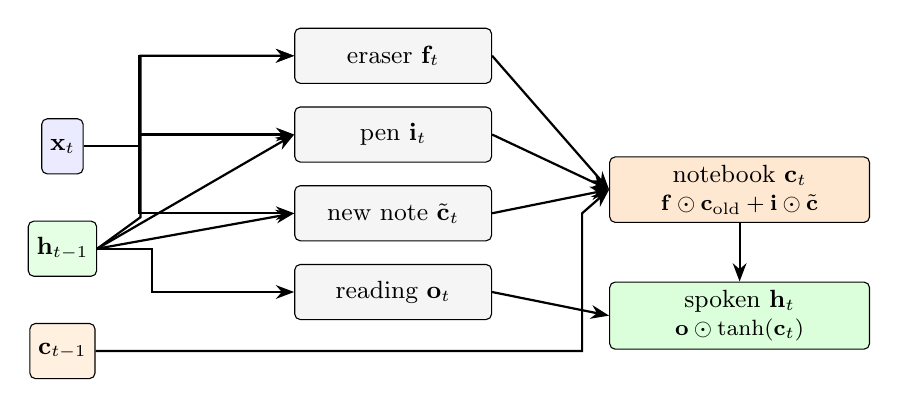
\begin{tikzpicture}[
  font=\small,
  >=Stealth,
  box/.style={draw, rounded corners=2pt, align=center,
              minimum height=0.7cm, inner sep=3pt},
  arr/.style={->, thick},
]
  \node[box, fill=blue!8] (x) at (0,0) {\(\mathbf{x}_t\)};
  \node[box, fill=green!10] (h) at (0,-1.3) {\(\mathbf{h}_{t-1}\)};
  \node[box, fill=orange!12] (cprev) at (0,-2.6) {\(\mathbf{c}_{t-1}\)};

  \node[box, fill=gray!8, minimum width=2.5cm] (f) at (4.2,1.15)
    {eraser \(\mathbf{f}_t\)};
  \node[box, fill=gray!8, minimum width=2.5cm] (i) at (4.2,0.15)
    {pen \(\mathbf{i}_t\)};
  \node[box, fill=gray!8, minimum width=2.5cm] (ct) at (4.2,-0.85)
    {new note \(\tilde{\mathbf{c}}_t\)};
  \node[box, fill=gray!8, minimum width=2.5cm] (o) at (4.2,-1.85)
    {reading \(\mathbf{o}_t\)};

  \draw[arr] (x.east) -- ++(0.7,0) |- (f.west);
  \draw[arr] (x.east) -- ++(0.7,0) |- (i.west);
  \draw[arr] (x.east) -- ++(0.7,0) |- (ct.west);
  \draw[arr] (h.east) -- ++(0.7,0) |- (o.west);
  \draw[arr] (h.east) -- (i.west);
  \draw[arr] (h.east) -- (ct.west);
  \draw[arr] (h.east) -- ++(0.55,0.4) |- (f.west);

  \node[box, fill=orange!18, minimum width=3.3cm] (cnew) at (8.6,-0.55)
    {notebook \(\mathbf{c}_t\)\\[-1pt]
     {\footnotesize \(\mathbf{f}\odot\mathbf{c}_{\mathrm{old}}
       +\mathbf{i}\odot\tilde{\mathbf{c}}\)}};
  \node[box, fill=green!14, minimum width=3.3cm] (hout) at (8.6,-2.15)
    {spoken \(\mathbf{h}_t\)\\[-1pt]
     {\footnotesize \(\mathbf{o}\odot\tanh(\mathbf{c}_t)\)}};

  \draw[arr] (f.east) -- (cnew.west);
  \draw[arr] (i.east) -- (cnew.west);
  \draw[arr] (ct.east) -- (cnew.west);
  \draw[arr] (cprev.east) -| (6.6,-2.6) -- (6.6,-0.85) -- (cnew.west);
  \draw[arr] (o.east) -- (hout.west);
  \draw[arr] (cnew.south) -- (hout.north);
\end{tikzpicture}
\caption{One LSTM step as a notebook. The eraser, pen, new note, and
reading switch are four separate dense layers of \(\mathbf{x}_t\) and
\(\mathbf{h}_{t-1}\). The notebook is updated by multiplying, not by
another \(W_h\). The spoken state is the only vector the rest of the
network hears.}
\label{fig:lstm-notebook}
\end{figure}

\subsection{One numerical step}

Take a one-number notebook so every product is ordinary multiplication.
Last step ended at \(c_{t-1}=4\) and \(h_{t-1}=0.5\). The new input is
\(x_t=1\). The weighted sums below are example weights, chosen so the
switches come out as easy numbers.

Eraser, mostly open:
\[
f_t=\sigma(1.0\cdot 1+1.0\cdot 0.5)=\sigma(1.5)\approx 0.82.
\]
Pen, half open: \(i_t=\sigma(0)=0.50\).
New note: \(\tilde{c}_t=\tanh(0.5)\approx 0.46\).
Reading switch, mostly open: \(o_t=\sigma(2.0)\approx 0.88\).

Update the notebook:
\[
c_t=0.82\times 4+0.50\times 0.46=3.28+0.23=3.51.
\]
The old \(4\) was mostly kept. The new note added a little. Then
\(\tanh(3.51)\approx 1\), so
\[
h_t=0.88\times 1\approx 0.88.
\]
The next step receives \(c_t=3.51\) and \(h_t=0.88\).

Three further settings of the same old notebook \(c_{t-1}=4\) show what the
switches are for.
\begin{itemize}[leftmargin=*]
  \item \textbf{Keep the old note.} Eraser open, pen shut:
        \(c_t=1\times 4+0\times(\text{anything})=4\). The new word arrives
        and the page does not change.
  \item \textbf{Erase and rewrite.} Eraser shut, pen open, new note \(-2\):
        \(c_t=0\times 4+1\times(-2)=-2\).
  \item \textbf{Remember it, but stay quiet.} Notebook holds \(4\), reading
        switch shut: \(h_t=0\times\tanh(4)=0\). The page still holds \(4\)
        for later. The spoken output this step is \(0\).
\end{itemize}

\subsection{Why the notebook is easier to train}

In a vanilla RNN the path back through time multiplies by \(W_h\) at every
step, which is the product in~\eqref{eq:linear-bptt}. On the notebook path
the backward pass multiplies by the eraser \(f_t\). If that switch stays
near \(1\), the old value passes through almost unchanged, step after step,
because the update is an addition
\(\mathbf{c}_t=\mathbf{f}_t\odot\mathbf{c}_{t-1}+\cdots\) rather than a
fresh multiplication by \(W_h\). A fact from word 2 can still affect word
50. The design was motivated by that goal, then checked empirically: LSTMs
train more reliably than vanilla RNNs. The particular gates, the separate
cell, and the \(\tanh\) on the candidate are part of that design, not a
derivation from a unique formula.

\begin{clarification}
Are \(W_{xf}\), \(W_{hf}\), \(W_{xi}\), \(W_{hi}\), and the other \(W\)'s
all learned?
\end{clarification}

Yes. Every one of them is a parameter, initialized randomly and updated by
gradient descent together with the rest of the network. Each gate has its
own pair, and the candidate note has a pair too. Nothing is shared between
them.

\begin{center}
\begin{tabular}{@{}llll@{}}
\toprule
Piece & Weights on \(\mathbf{x}_t\) & Weights on \(\mathbf{h}_{t-1}\) & Bias \\
\midrule
eraser \(\mathbf{f}_t\) & \(W_{xf}\) & \(W_{hf}\) & \(\mathbf{b}_f\) \\
pen \(\mathbf{i}_t\) & \(W_{xi}\) & \(W_{hi}\) & \(\mathbf{b}_i\) \\
new note \(\tilde{\mathbf{c}}_t\) & \(W_{xc}\) & \(W_{hc}\) & \(\mathbf{b}_c\) \\
reading switch \(\mathbf{o}_t\) & \(W_{xo}\) & \(W_{ho}\) & \(\mathbf{b}_o\) \\
\bottomrule
\end{tabular}
\end{center}

That is 8 matrices and 4 bias vectors for one LSTM cell. Training is the
same loop as the vanilla RNN. The loss is still the next-word
cross-entropy. Backpropagation through time sends a gradient to every
matrix that participated. \(W_{xf}\) moves when changing the eraser makes
the next-word loss smaller. \(W_{xi}\) moves when changing the pen helps.
Each matrix learns its own job because each one sits on a different path
into \(\mathbf{c}_t\) and \(\mathbf{h}_t\).

%----------------------------------------------------------------------
\section{Deep and Bidirectional RNNs}
%----------------------------------------------------------------------

Two extensions are worth having in hand before the tasks.

\textbf{Deep RNNs} stack layers. The first layer reads the input. Each
later layer reads the hidden state of the layer below it, at the same time
step, together with its own previous state:
\[
\mathbf{h}_t^{(1)}
=
f^{(1)}(\mathbf{x}_t,\mathbf{h}_{t-1}^{(1)}),
\qquad
\mathbf{h}_t^{(2)}
=
f^{(2)}(\mathbf{h}_t^{(1)},\mathbf{h}_{t-1}^{(2)}),
\quad\ldots
\]
Stacking here is the same idea as stacking feedforward layers. There are
simply more indices.

\textbf{Bidirectional RNNs} run two layers with separate parameters, one
left to right and one right to left:
\[
\overrightarrow{\mathbf{h}}_t
=
\overrightarrow{f}(\mathbf{x}_t,\overrightarrow{\mathbf{h}}_{t-1}),
\qquad
\overleftarrow{\mathbf{h}}_t
=
\overleftarrow{f}(\mathbf{x}_t,\overleftarrow{\mathbf{h}}_{t+1}).
\]
Concatenating them at a step gives a vector that has seen the full past and
the full future. That is the wrong tool for predicting the next element,
because the future is what the model is trying to predict. It is the right
tool when the whole input sequence is already in hand, for example when the
job is to classify it.

%----------------------------------------------------------------------
\section{Language Modeling and Sequence Classification}
%----------------------------------------------------------------------

\subsection{Language modeling and teacher forcing}

Predicting \(p(\mathbf{x}_t\mid\mathbf{x}_{t-1},\ldots,\mathbf{x}_1)\) is
\textbf{language modeling}, and a model trained to do it is a language
model. Training uses \textbf{teacher forcing}: to predict \(\mathbf{x}_t\),
feed the true prefix up through \(\mathbf{x}_{t-1}\), regardless of what
the model would have predicted for the earlier positions, and train it to
match the true \(\mathbf{x}_t\).

A trained language model is useful in the two ways from
Section~\ref{sec:vanilla}'s setup. It can sample new sequences
autoregressively. It can also score an existing sequence, by multiplying
the next-element probabilities along the observed tokens, and so say
whether that sequence looks typical under the model.

\subsection{Sequence classification}

Sequence classification predicts one label from the whole input,
\(p(\mathbf{y}\mid\mathbf{x}_1,\ldots,\mathbf{x}_T)\). Run the recurrence to
the end and read a single dense layer off the final state:
\[
\mathbf{h}_t=f(\mathbf{x}_t,\mathbf{h}_{t-1}),
\qquad
\mathbf{o}=W_o\mathbf{h}_T+\mathbf{b}_o.
\]
The final state \(\mathbf{h}_T\) is the summary of the entire input. When
the full sequence is available at prediction time, a bidirectional net can
combine the final forward state \(\overrightarrow{\mathbf{h}}_T\) with the
final backward state \(\overleftarrow{\mathbf{h}}_1\). Document topic,
sentiment of a review, and spam detection are all this pattern: a sequence
of word embeddings in, one class out.

%----------------------------------------------------------------------
\section{Sequence-to-Sequence and the Decoder LSTM}
\label{sec:seq2seq}
%----------------------------------------------------------------------

Sequence-to-sequence learning generates an output sequence from an input
sequence. The standard example is translation: \(\mathbf{x}\) is an English
sentence and \(\mathbf{y}\) is its French translation. The output is still
produced autoregressively, but each output word is conditioned on the
output so far \emph{and} on the full input. Writing the output clock as
\(t'\),
\[
p(\mathbf{y}_{t'}
\mid
\mathbf{y}_{t'-1},\ldots,\mathbf{y}_1,\;
\mathbf{x}_T,\ldots,\mathbf{x}_1).
\]

The lecture builds this from two RNNs (Sutskever et al., 2014).
\begin{enumerate}[leftmargin=*]
  \item An \textbf{encoder} reads the input,
        \(\mathbf{h}_t=f(\mathbf{x}_t,\mathbf{h}_{t-1})\), and produces a
        sequence of hidden states. The encoder may be bidirectional,
        because the whole input is available.
  \item The \textbf{context} is the encoder's final state,
        \(\mathbf{c}=\mathbf{h}_T\). One vector summarizes the input
        sentence.
  \item A \textbf{decoder} generates the output,
        \begin{equation}
        \label{eq:decoder}
        \mathbf{s}_{t'}
        =
        g(\mathbf{y}_{t'-1},\;\mathbf{s}_{t'-1},\;\mathbf{c}).
        \end{equation}
        Its state predicts \(\mathbf{y}_{t'}\). The decoder is not
        bidirectional: it writes left to right.
\end{enumerate}

Generation starts by feeding a beginning-of-sequence token, a token with no
meaning in the language and a definite meaning to the model. It stops when
the decoder emits an end-of-sequence token.

\begin{clarification}
Which line is the decoder?
\end{clarification}

The decoder is the whole of \(g\) in~\eqref{eq:decoder}, not one gate
inside it. When \(g\) is a single-layer LSTM, one call of \(g\) runs
\eqref{eq:lstm-f}--\eqref{eq:lstm-h} and returns the new spoken state.
That spoken state is \(\mathbf{s}_{t'}=\mathbf{h}_{t'}\). A dense layer
then turns \(\mathbf{h}_{t'}\) into a distribution over the next output
word. The encoder is a separate network that already ran and produced
\(\mathbf{c}\).

The three arguments of \(g\) land in different places.
\begin{itemize}[leftmargin=*]
  \item \(\mathbf{y}_{t'-1}\) is the previous output word. It enters as its
        embedding.
  \item \(\mathbf{s}_{t'-1}\) is the decoder's own memory from the previous
        output step. For an LSTM that memory is the pair
        \((\mathbf{h}_{t'-1},\mathbf{c}_{t'-1})\): spoken state and
        notebook. The notebook here is the LSTM cell, not the encoder
        context. The lecture uses \(\mathbf{c}\) for the context, so the
        rest of this section keeps \(\mathbf{c}\) for the encoder vector
        and \(\mathbf{h}\) for the spoken state.
  \item \(\mathbf{c}\) is the encoder summary. The two options below put it
        in different slots of \(g\).
\end{itemize}

There are two standard ways to make \(g\) depend on \(\mathbf{c}\).
\begin{enumerate}[leftmargin=*]
  \item Concatenate \(\mathbf{c}\) with the embedding of the previous
        output word at every step:
        \[
          \operatorname{concat}\bigl(
            \operatorname{embed}(\mathbf{y}_{t'-1}),\,\mathbf{c}
          \bigr).
        \]
        The context is re-injected on every output word. The initial spoken
        state can be zeros.
  \item Set the decoder's initial spoken state to the context,
        \(\mathbf{s}_0=\mathbf{c}\). This uses \(\mathbf{c}\) once. Later
        steps see the input sentence only because that starting memory was
        carried forward. The usual other choices for an initial state are
        all zeros, or a learned vector.
\end{enumerate}

\subsection{Worked count: two ways to feed the context}

\begin{clarification}
The decoder is a single-layer LSTM with hidden size 8 and 5-dimensional
input embeddings, with biases everywhere. The encoder context \(\mathbf{c}\)
has dimension 8. In Option~A, \(\mathbf{c}\) is concatenated to the
embedding of the previous output token at every step, and the initial
hidden state is zero. In Option~B, the inputs are just the embeddings, and
the initial hidden state is set to \(\mathbf{c}\). How many more parameters
does the LSTM have in Option~A than in Option~B?
\end{clarification}

The answer is \(256\). Concatenating the context makes the decoder input
wider, so the four matrices that multiply that input grow. Copying
\(\mathbf{c}\) into the initial spoken state adds no weights.

\paragraph{What \(h\) is, and why the matrices in front of it stay put.}
Hidden size 8 means the spoken state is always these eight numbers:
\[
\mathbf{h}
=
[h_1,h_2,h_3,h_4,h_5,h_6,h_7,h_8].
\]
A matrix that multiplies \(\mathbf{h}\) needs one column per entry of
\(\mathbf{h}\). There are eight entries, and the product must be eight gate
values, so each of \(W_{hf}\), \(W_{hi}\), \(W_{hc}\), and \(W_{ho}\) is
\(8\times 8\) in both options.

Option~A does not lengthen \(\mathbf{h}\). It lengthens a different vector,
the decoder input \(\mathbf{x}\). Let the previous output embedding be
\([e_1,\ldots,e_5]\) and the context be \([c_1,\ldots,c_8]\).
\begin{align*}
\text{Option B:}&\quad
\mathbf{x}=[e_1,\ldots,e_5]
\quad\text{(length 5)},
&&
\mathbf{h}_0=\mathbf{c}.
\\
\text{Option A:}&\quad
\mathbf{x}=[e_1,\ldots,e_5,\,c_1,\ldots,c_8]
\quad\text{(length \(5+8=13\))},
&&
\mathbf{h}_0=\mathbf{0}.
\end{align*}
Setting \(\mathbf{h}_0=\mathbf{c}\) is an assignment. The context is
already 8 numbers, the same length as the spoken state, so it can be copied
straight into \(\mathbf{h}_0\). There is no new matrix. Option~A's
\(\mathbf{h}_0=\mathbf{0}\) is a constant. From the next step on,
\(\mathbf{h}\) is still 8 numbers produced by the LSTM, in both options.

\paragraph{Where the 4 matrices and the extra columns come from.}
Look back at \eqref{eq:lstm-f}--\eqref{eq:lstm-c}. Four lines multiply the
decoder input \(\mathbf{x}\):
\[
W_{xf},\qquad W_{xi},\qquad W_{xc},\qquad W_{xo}.
\]
Those are the four matrices that change. The other four,
\(W_{hf},W_{hi},W_{hc},W_{ho}\), multiply \(\mathbf{h}\), whose length stays
8.

A matrix can multiply a vector only when it has one column per entry of
that vector. One row of \(W_{xf}\) in Option~B has five weights, one per
embedding coordinate:
\[
[w_1\ w_2\ w_3\ w_4\ w_5]
\cdot
[e_1\ e_2\ e_3\ e_4\ e_5].
\]
Option~A glues on eight context numbers, so the same row needs eight more
weights:
\[
[w_1\ \cdots\ w_5\ \ u_1\ \cdots\ u_8]
\cdot
[e_1\ \cdots\ e_5\ \ c_1\ \cdots\ c_8].
\]
The \(u\)'s are the extra columns. The eraser has 8 rows, one per notebook
slot:
\[
8\text{ rows}\times 8\text{ new columns}=64.
\]
One gate therefore has
\[
8\times 13-8\times 5=64
\]
more weights in Option~A. The pen, the new note, and the reading switch are
separate matrices of the same shape, so each contributes its own 64:
\[
4\times 64=256.
\]

The biases do not move this difference. Each bias is added after the
multiply and has one number per notebook slot, so each gate has 8 bias
parameters in both options. The 5-dimensional embedding table is the same
size in both options, and the question does not give a vocabulary size, so
the embedding table and the final softmax are not part of the comparison.
The question asks only about the LSTM.

Full totals, as a check:
\begin{align*}
\text{Option A}
&=
4(8\cdot 13)+4(8\cdot 8)+4(8)
=
416+256+32
=
704,\\
\text{Option B}
&=
4(8\cdot 5)+4(8\cdot 8)+4(8)
=
160+256+32
=
448.
\end{align*}
\[
704-448=256.
\]
The \(256\) recurrent weights and the \(32\) biases sit in both totals, so
they cancel. Only the widened input matrices remain:
\(416-160=256\).

%----------------------------------------------------------------------
\section{Cheat Sheet}
%----------------------------------------------------------------------

\begin{enumerate}[leftmargin=*]
  \item \textbf{Sequence.} Ordered random variables. The chain rule writes
        the joint as next-element conditionals. One model of
        \(p(x_t\mid x_{<t})\) scores sequences and samples them
        autoregressively.
  \item \textbf{Lookup table.} A separate categorical distribution per
        prefix costs
        \(\bigl((|V|^T-1)/(|V|-1)\bigr)\times(|V|-1)\)
        free parameters. For \(|V|=3\), \(T=4\), that is \(40\times 2=80\).
        The \(2\) is ``probabilities minus the constraint that they sum to
        1.''
  \item \textbf{Embedding.} One-hot times \(W\) copies out one column.
        That column is the word embedding, and in this lecture \(W\) is the
        RNN's input matrix \(W_x\), trained by next-word cross-entropy.
        Word2vec learns a similar column with a shallow window objective and
        then keeps the columns alone.
  \item \textbf{Vanilla RNN.}
        \(\mathbf{h}_t=\sigma(W_x\mathbf{x}_t+W_h\mathbf{h}_{t-1}+\mathbf{b}_h)\).
        Any length, fixed parameter list. \(\mathbf{h}_t\) summarizes the
        prefix.
  \item \textbf{BPTT.} Unroll, then backpropagate. The recurrent term has a
        direct path and an indirect path through \(\mathbf{h}_{t-1}\). In
        the linear case the indirect path multiplies by \(W_h\) once per
        step, so gradients explode or vanish.
        Scalar check: \(w=-2\), loss \(\sum_{t=1}^{6}h_t\), gives
        \(\partial\mathcal{L}/\partial x_1=1+w+\cdots+w^5=-21\).
  \item \textbf{ReLU cut.} A negative pre-activation has slope \(0\) and
        stops the chain. In the worked ReLU RNN,
        \(\mathrm{d}\mathcal{L}/\mathrm{d}w=12\), with the early chain
        killed at the step whose pre-activation is \(-2\).
  \item \textbf{LSTM notebook.} \(\mathbf{c}_t\) is the private page,
        \(\mathbf{h}_t\) is what is said aloud. Eraser \(\mathbf{f}_t\), pen
        \(\mathbf{i}_t\), new note \(\tilde{\mathbf{c}}_t\), reading switch
        \(\mathbf{o}_t\). Eight matrices and four biases, all learned,
        none shared. The backward path through the page multiplies by
        \(\mathbf{f}_t\); a forget gate near \(1\) carries a memory across
        many steps.
  \item \textbf{Uses.} Language modeling with teacher forcing; sequence
        classification from \(\mathbf{h}_T\) (bidirectional when the whole
        input is available); sequence-to-sequence with an encoder context
        \(\mathbf{c}=\mathbf{h}_T\) fed to a left-to-right decoder.
  \item \textbf{Decoder parameter gap.} Concatenating an 8-dimensional
        context onto a 5-dimensional embedding widens each of the four
        input matrices \(W_{x*}\) from \(8\times 5\) to \(8\times 13\).
        Four times \(8\times 8\) extra columns is \(256\). The matrices in
        front of \(\mathbf{h}\) stay \(8\times 8\) because \(\mathbf{h}\)
        stays length 8. Setting \(\mathbf{h}_0=\mathbf{c}\) adds no
        weights.
\end{enumerate}

\noindent\textbf{Remember:}
\emph{a one-hot vector points at a column; that column is the embedding,
and the RNN learns it. The hidden state is a shared-weight stand-in for the
whole prefix. Backpropagation through time multiplies by the same \(W_h\)
at every step. The LSTM's notebook is updated by addition and by dimmer
switches, so a memory can sit still. In a decoder, widening the input
widens only the matrices that multiply the input.}

%----------------------------------------------------------------------
\section*{References}
%----------------------------------------------------------------------

\begin{itemize}[leftmargin=*]
  \item Hochreiter, S., and Schmidhuber, J. (1997).
        Long Short-Term Memory. \emph{Neural Computation}, 9(8), 1735--1780.
  \item Mikolov, T., Sutskever, I., Chen, K., Corrado, G., and Dean, J.
        (2013). Distributed Representations of Words and Phrases and Their
        Compositionality. \emph{NeurIPS}.
  \item Sutskever, I., Vinyals, O., and Le, Q.\ V. (2014).
        Sequence to Sequence Learning with Neural Networks. \emph{NeurIPS}.
\end{itemize}

\end{document}
